
% % \paragraph{Sơ đồ tuần tự Luồng xử lý tài liệu}

% % Luồng nghiệp vụ này mô tả vòng đời của tài liệu khi người dùng tải lên hệ thống, lưu trữ tệp tin, trích xuất nội dung và lưu trữ dữ liệu vector phục vụ tính năng RAG.

% % \begin{figure}[H]
% % \centering
% % 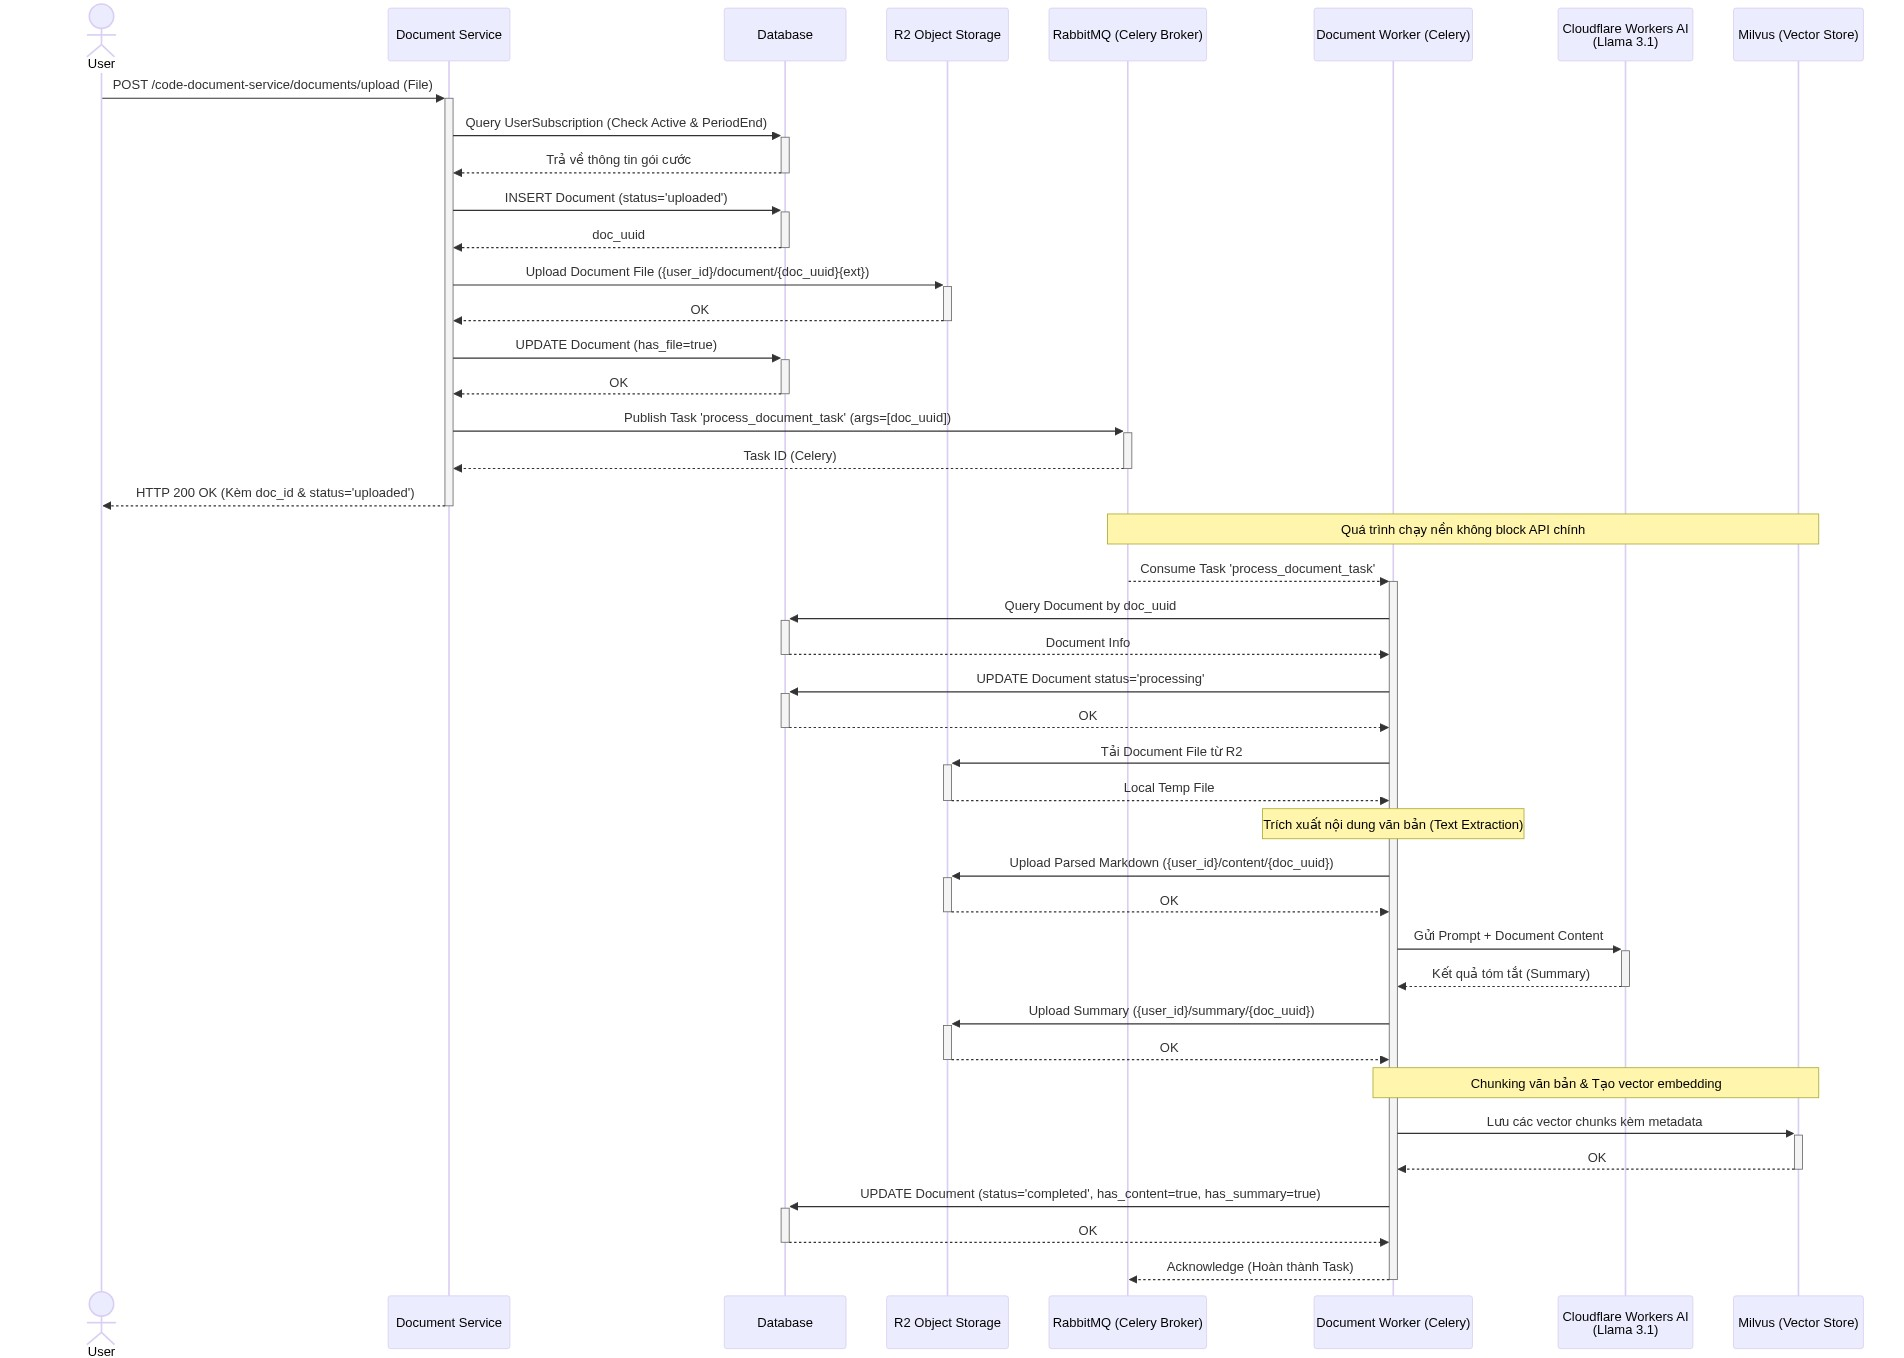
\includegraphics[scale = 0.18]{pictures/Sequence-document.png}
% % \caption{Sơ đồ tuần tự Luồng xử lý tài liệu}
% % \end{figure}

% % \subparagraph{Các thành phần tham gia}

% % \begin{table}[H]
% % \centering
% % \renewcommand{\arraystretch}{1.3}
% % \begin{tabular}{|l|l|p{5cm}|}
% % \hline
% % \textbf{Thành phần} & \textbf{Phân loại} & \textbf{Vai trò trong hệ thống} \\ \hline
% % User & Actor & Người dùng thực hiện tải lên tài liệu và nhận phản hồi trạng thái từ hệ thống. \\ \hline
% % Document Service & Microservice & Dịch vụ chính tiếp nhận yêu cầu, kiểm qua gói dịch vụ người dùng. \\ \hline
% % Database & Database & Cơ sở dữ liệu kiểm tra thông tin gói cước người dùng (UserSubscription) và lưu trữ trạng thái của tài liệu. \\ \hline
% % R2 Object Storage & Object Storage & Kho lưu trữ dùng để lưu trữ file tài liệu. \\ \hline
% % RabbitMQ (Celery Broker) & Message Broker & Hàng đợi tác vụ (Task Queue) cho Celery, tiếp nhận và phân phối các công việc. \\ \hline
% % Document Worker (Celery) & Worker Service & Tiến trình xử lý tải file, trích xuất text, gọi dịch vụ AI và đồng bộ dữ liệu vào Vector Store. \\ \hline
% % Cloudflare Workers AI & External Service / AI Engine & Dịch vụ trí tuệ nhân tạo tiếp nhận prompt và nội dung tài liệu từ Worker để xử lý và trả về kết quả tóm tắt (Summary). \\ \hline
% % Milvus (Vector Store) & Vector Database & Cơ sở dữ liệu vector chịu trách nhiệm lưu trữ các đoạn văn bản (chunks) kèm theo nhúng (embeddings) và metadata để phục vụ tìm kiếm ngữ nghĩa (RAG). \\ \hline
% % \end{tabular}
% % \caption{Danh sách các thành phần và vai trò trong Sơ đồ tuần tự Luồng xử lý tài liệu}
% % \label{tab:system_components_document}
% % \end{table}

% % \subparagraph{Mô tả tổng quan}

% % \begin{itemize}
% % \item Người dùng gửi yêu cầu tải lên file văn bản.
% % \item Dịch vụ tài liệu kiểm tra điều kiện bảng UserSubscription trong Database.
% % \item Dịch vụ tài liệu lưu file vào R2 Object Storage.
% % \item Dịch vụ tài liệu đẩy thông tin công việc vào hệ thống nhắn tin RabbitMQ.
% % \item Dịch vụ tài liệu trả ngay kết quả tải lên thành công cho người dùng.
% % \item Document Worker tải file từ R2 Object Storage
% % \item Document Worker xử lý tóm tắt và RAG file tài liệu với Cloudflare Workers AI, Vector Database
% % \item Document Worker cập nhật thông tin trong database
% % \end{itemize}
